\section{Results}

\subsection{Effect of Varying Temperature}
For each Model$\times$Probe$\times$Graph configuration, we compared macro-F$_1$ across temperatures using pairwise Welch's $t$-tests (unequal variances) for the three temperature values: $0$ vs.\ $0.2$, $0.2$ vs.\ $0.5$, and $0$ vs.\ $0.5$. Within each configuration we applied Holm–Bonferroni correction across the three tests; statistical significance is denoted as * ($p_{\text{adj}}{<}.05$), ** ($p_{\text{adj}}{<}.01$), and *** ($p_{\text{adj}}{<}.001$). Effect sizes (Cohen’s $d$) were computed for all comparisons.

Because each temperature condition is represented by a single run per configuration (i.e., $n{=}1$ per temperature), inferential tests were of low statistical power and produced no adjusted $p$-values below $.05$; consequently, no cells received a significance marker after Holm correction. We therefore report directional patterns descriptively. Across all 84 configurations, increasing temperature from $0{\to}0.5$ reduced macro-F$_1$ in 52 cases, increased it in 23, and left it unchanged in 9 (median $\Delta=-0.02$). The attenuation with higher $T$ was more pronounced on Probe 1 (28 decreases, 9 increases; median $\Delta=-0.03$) than Probe 2 (24 decreases, 14 increases; median $\Delta=-0.01$). By graph condition, $\mathbb{G}_1$ was most temperature-stable (balanced 7 increases/7 decreases; median $\Delta\approx0$), whereas $\mathbb{G}_2$, $\mathbb{G}_3$, and $\mathbb{G}_1$+$\mathbb{G}_2$(+$\mathbb{G}_3$) skewed toward decreasing values, however, it was small (median $\Delta\in[-0.03,-0.015]$). By model, \texttt{Anthropic.Claude-3-Haiku} showed the mildest tendency to improve with temperature (median $\Delta{=}+0.005$), while \texttt{Mistral-7B-Instruct-v0.3} exhibited the largest typical drop (median $\Delta{=}-0.12$). Illustratively, the largest decrease occurred for \texttt{Mistral-7B-Instruct-v0.3} on Probe~1 across several graphs ($\Delta_{0{\to}0.5}\in[-0.25,-0.21]$), whereas a notable increase was observed for \texttt{Mixtral-8x7B-v0.1} (No-RAG, Probe 2; $\Delta_{0{\to}0.5}{=}+0.09$).

On the domain of single-run estimations (no stars beyond the Holm adjustment), on the graphs of macro-F$_1$, the trend of higher decoding temperature is, in most cases, downward, particularly Probe~1 and non-$\mathbb{G}_1$ graphs. When stability is preferred, $T{=}0$ is the safest default; small exploration at $T{=}0.2$ may be helpful in some environments, but $T{=}0.5$ tends to worsen the accuracy. Accordingly, we take an averaged value of each of these temperatures.

\begin{table}[t]
\centering
\scriptsize
\caption{Temperature sensitivity by graph (macro-F$_1$). Counts across all Model$\times$Probe settings; $\Delta$ is median change from $T{=}0$ to $0.5$.}
\begin{tabular}{lrrrr}
\hline
Graph & \# Increases & \# Decreases & \# No change & Median $\Delta$ (0$\to$0.5) \\
\hline
$\mathbb{G}_1$         & 7  & 7  & 0 &  0.00 \\
$\mathbb{G}_1$+$\mathbb{G}_2$      & 3  & 10 & 1 & -0.03 \\
$\mathbb{G}_1$+$\mathbb{G}_2$+$\mathbb{G}_3$   & 3  & 9  & 2 & -0.03 \\
$\mathbb{G}_2$         & 3  & 10 & 1 & -0.03 \\
$\mathbb{G}_3$         & 3  & 8  & 3 & -0.02 \\
No-RAG     & 4  & 8  & 2 & -0.02 \\
\hline
\end{tabular}
\label{tab:temp-by-graph}
\end{table}

% \noindent\emph{Significance notation:} * $p_{\text{adj}}{<}.05$, ** $p_{\text{adj}}{<}.01$, *** $p_{\text{adj}}{<}.001$ (Holm–Bonferroni across within-configuration contrasts).


\begin{table*}[ht] 
\centering 
\caption{Results of Probe 1, Averaged across the three temperatures (0.0, 0.2 and 0.5)}
\label{tab:probe1} 
\scriptsize 
\begin{tabular}{l l c c c c c c}
\hline
\multicolumn{2}{c}{} & \multicolumn{6}{c}{Systems} \\
\cline{3-8}
Model & Metric & $\mathbb{G}_1$ & $\mathbb{G}_1$+$\mathbb{G}_2$ & $\mathbb{G}_1$+$\mathbb{G}_2$+$\mathbb{G}_3$ & $\mathbb{G}_2$ & $\mathbb{G}_3$ & No-RAG \\
\hline
\multirow{2}{*}{Anthropic.Claude-3-Haiku} & Acc/ F$_{1Micro}$ & 0.84 / 0.84 & \textbf{0.92} / \textbf{0.92} & \textbf{0.93} / \textbf{0.93} & \textbf{0.93} / \textbf{0.93} & 0.89 / 0.89 & \textbf{0.96} / \textbf{0.96} \\

& Macro P/R/F$_1$ & 0.87 / 0.84 / 0.84 & \textbf{0.93} / \textbf{0.93} / \textbf{0.93} & \textbf{0.94} / \textbf{0.93} / \textbf{0.93} & \textbf{0.94} / \textbf{0.94} / \textbf{0.93} & 0.91 / 0.90 / 0.90 & 0.91 / 0.91 / 0.91 \\
\hline
\multirow{2}{*}{GPT-OSS-20B} & Acc/ F$_{1Micro}$ & \textbf{0.87} / \textbf{0.87} & 0.85 / 0.85 & 0.82 / 0.82 & 0.82 / 0.82 & 0.84 / 0.84 & 0.91 / 0.91 \\
& Macro P/R/F$_1$ & \textbf{0.88} / \textbf{0.87} / \textbf{0.87} & 0.87 / 0.86 / 0.86 & 0.85 / 0.83 / 0.82 & 0.84 / 0.82 / 0.82 & 0.87 / 0.85 / 0.85 & 0.92 / 0.92 / 0.91 \\
\hline
\multirow{2}{*}{Llama-3.1-8B-Instruct} & Acc/ F$_{1Micro}$ & 0.69 / 0.69 & 0.63 / 0.63 & 0.65 / 0.65 & 0.66 / 0.66 & 0.67 / 0.67 & 0.83 / 0.83 \\
& Macro P/R/F$_1$ & 0.76 / 0.66 / 0.67 & 0.69 / 0.62 / 0.62 & 0.74 / 0.63 / 0.65 & 0.71 / 0.65 / 0.65 & 0.74 / 0.65 / 0.66 & 0.85 / 0.82 / 0.83 \\
\hline
\multirow{2}{*}{Llama-3.3-70B-Instruct} & Acc/ F$_{1Micro}$ & 0.86 / 0.86 & 0.91 / 0.91 & 0.92 / 0.92 & 0.91 / 0.91 & \textbf{0.92} / \textbf{0.92} & 0.95 / 0.95 \\
& Macro P/R/F$_1$ & 0.72 / 0.71 / 0.71 & 0.91 / 0.91 / 0.91 & 0.93 / 0.92 / 0.92 & 0.91 / 0.90 / 0.90 & \textbf{0.92} / \textbf{0.92} / \textbf{0.92} & \textbf{0.96} / \textbf{0.96} / \textbf{0.96} \\
\hline
\multirow{2}{*}{Mistral-7B-Instruct-v0.3} & Acc/ F$_{1Micro}$ & 0.67 / 0.67 & 0.68 / 0.68 & 0.69 / 0.69 & 0.73 / 0.73 & 0.72 / 0.72 & 0.67 / 0.67 \\
& Macro P/R/F$_1$ & 0.79 / 0.67 / 0.70 & 0.75 / 0.69 / 0.70 & 0.77 / 0.70 / 0.71 & 0.78 / 0.73 / 0.74 & 0.78 / 0.72 / 0.73 & 0.78 / 0.66 / 0.69 \\
\hline
\multirow{2}{*}{Mixtral-8x7B-v0.1} & Acc/ F$_{1Micro}$ & 0.83 / 0.83 & 0.83 / 0.83 & 0.87 / 0.87 & 0.88 / 0.88 & 0.84 / 0.84 & 0.79 / 0.79 \\
& Macro P/R/F$_1$ & 0.86 / 0.83 / 0.84 & 0.82 / 0.80 / 0.80 & 0.88 / 0.87 / 0.87 & 0.90 / 0.89 / 0.89 & 0.86 / 0.85 / 0.84 & 0.85 / 0.79 / 0.80 \\
\hline
\multirow{2}{*}{Qwen2.5-32B-Instruct} & Acc/ F$_{1Micro}$ & 0.85 / 0.85 & 0.90 / 0.90 & 0.89 / 0.89 & 0.89 / 0.89 & 0.87 / 0.87 & 0.91 / 0.91 \\
& Macro P/R/F$_1$ & 0.84 / 0.84 / 0.84 & 0.90 / 0.89 / 0.89 & 0.89 / 0.88 / 0.88 & 0.89 / 0.87 / 0.88 & 0.87 / 0.87 / 0.87 & 0.92 / 0.90 / 0.91 \\
\hline
\end{tabular}
\end{table*}




\begin{table*}[ht] 
\centering 
\caption{Results of Probe 2, Averaged across the three temperatures (0.0, 0.2 and 0.5)}
\label{tab:probe2} 
\scriptsize 
\begin{tabular}{l l c c c c c c}
\hline
\multicolumn{2}{c}{} & \multicolumn{6}{c}{Systems} \\
\cline{3-8}
Model & Metric & $\mathbb{G}_1$ & $\mathbb{G}_1$+$\mathbb{G}_2$ & $\mathbb{G}_1$+$\mathbb{G}_2$+$\mathbb{G}_3$ & $\mathbb{G}_2$ & $\mathbb{G}_3$ & No-RAG \\
\hline
\multirow{2}{*}{Anthropic.Claude-3-Haiku} & Acc/ F$_{1Micro}$ & \textbf{0.58} / \textbf{0.58} & \textbf{0.60} / \textbf{0.60} & \textbf{0.62} / \textbf{0.62} & 0.61 / 0.61 & 0.53 / 0.53 & 0.61 / 0.61 \\
& Macro P/R/F1 & 0.53 / 0.52 / 0.50 & 0.57 / 0.57 / \textbf{0.55} & \textbf{0.60} / \textbf{0.60} / \textbf{0.57} & 0.56 / 0.55 / 0.54 & 0.50 / 0.49 / 0.47 & 0.54 / 0.55 / 0.55 \\
\hline
\multirow{2}{*}{GPT-OSS-20B} & Acc/ F$_{1Micro}$ & 0.46 / 0.46 & 0.50 / 0.50 & 0.48 / 0.48 & 0.50 / 0.50 & 0.44 / 0.44 & 0.43 / 0.43 \\
& Macro P/R/F1 & 0.56 / 0.45 / 0.45 & 0.56 / 0.47 / 0.46 & 0.57 / 0.47 / 0.46 & \textbf{0.63} / 0.51 / 0.48 & \textbf{0.54} / 0.46 / 0.41 & 0.49 / 0.42 / 0.39 \\
\hline
\multirow{2}{*}{Llama-3.1-8B-Instruct} & Acc/ F$_{1Micro}$ & 0.53 / 0.53 & 0.51 / 0.51 & 0.48 / 0.48 & 0.56 / 0.56 & \textbf{0.54} / \textbf{0.54} & 0.61 / 0.61 \\
& Macro P/R/F1 & 0.44 / 0.41 / 0.41 & 0.47 / 0.41 / 0.42 & 0.40 / 0.38 / 0.37 & 0.52 / 0.44 / 0.45 & 0.45 / 0.41 / 0.40 & 0.51 / 0.50 / 0.50 \\
\hline
\multirow{2}{*}{Llama-3.3-70B-Instruct} & Acc/ F$_{1Micro}$ & \textbf{0.58} / \textbf{0.58} & 0.54 / 0.54 & 0.54 / 0.54 & 0.59 / 0.59 & 0.52 / 0.52 & 0.56 / 0.56 \\
& Macro P/R/F1 & 0.52 / 0.51 / 0.51 & 0.47 / 0.47 / 0.47 & 0.51 / 0.50 / 0.49 & 0.53 / 0.52 / 0.52 & 0.48 / 0.49 / \textbf{0.48} & 0.52 / 0.49 / 0.49 \\
\hline
\multirow{2}{*}{Mistral-7B-Instruct-v0.3} & Acc/ F$_{1Micro}$ & 0.36 / 0.36 & 0.40 / 0.40 & 0.39 / 0.39 & 0.44 / 0.44 & 0.35 / 0.35 & 0.38 / 0.38 \\
& Macro P/R/F1 & 0.32 / 0.26 / 0.23 & 0.46 / 0.31 / 0.29 & 0.36 / 0.28 / 0.25 & 0.46 / 0.34 / 0.33 & 0.38 / 0.27 / 0.24 & 0.40 / 0.31 / 0.29 \\
\hline
\multirow{2}{*}{Mixtral-8x7B-v0.1} & Acc/ F$_{1Micro}$ & 0.47 / 0.47 & 0.58 / 0.58 & 0.57 / 0.57 & 0.56 / 0.56 & 0.47 / 0.47 & 0.46 / 0.46 \\
& Macro P/R/F1 & 0.44 / 0.43 / 0.42 & 0.55 / 0.54 / 0.54 & 0.51 / 0.50 / 0.50 & 0.52 / 0.51 / 0.51 & 0.45 / 0.44 / 0.43 & 0.47 / 0.39 / 0.39 \\
\hline
\multirow{2}{*}{Qwen2.5-32B-Instruct} & Acc/ F$_{1Micro}$ & 0.56 / 0.56 & 0.56 / 0.56 & 0.55 / 0.55 & \textbf{0.64} / \textbf{0.64} & 0.51 / 0.51 & \textbf{0.65} / \textbf{0.65} \\
& Macro P/R/F1 & \textbf{0.60} / \textbf{0.60} / \textbf{0.54} & \textbf{0.59} / \textbf{0.61} / \textbf{0.55} & 0.53 / 0.55 / 0.52 & 0.62 / \textbf{0.65} / \textbf{0.61} & 0.51 / \textbf{0.53} / \textbf{0.48} & \textbf{0.61} / \textbf{0.63} / \textbf{0.60} \\
\hline
\end{tabular}
\end{table*}

\begin{figure*}[ht]
  \centering
  \begin{subfigure}{0.49\linewidth}
    \centering
    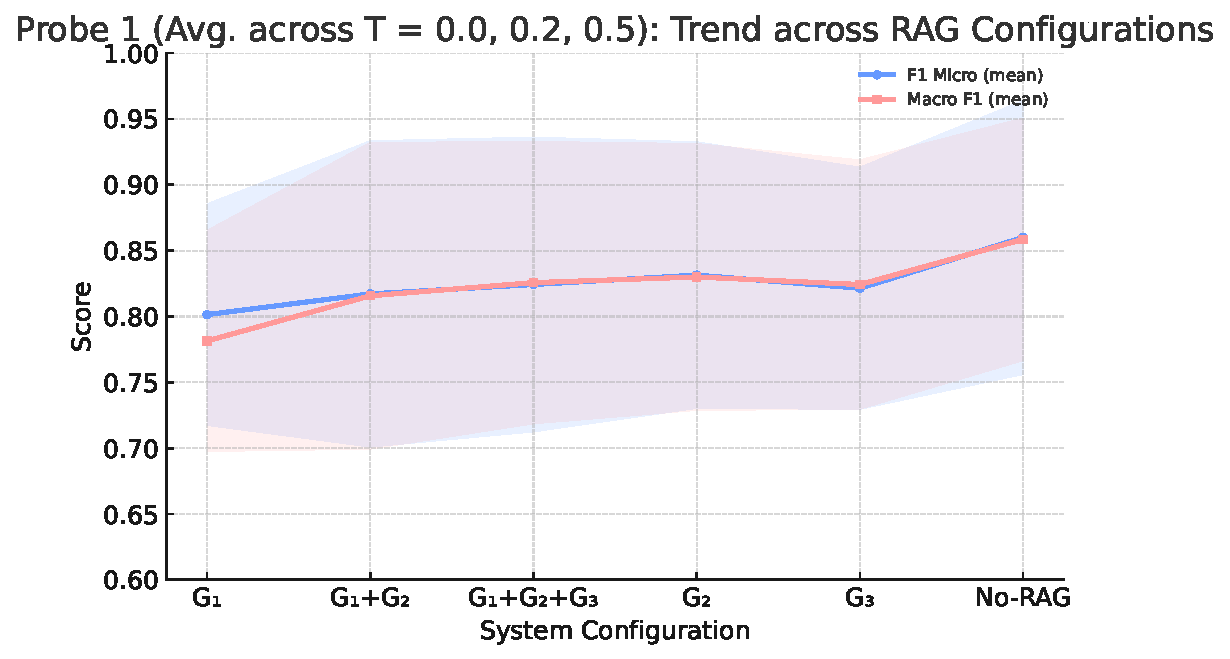
\includegraphics[width=\linewidth]{images/probe1_trend.pdf}
    \caption{Probe 1}
    \label{fig:probe1}
  \end{subfigure}\hfill
  \begin{subfigure}{0.49\linewidth}
    \centering
    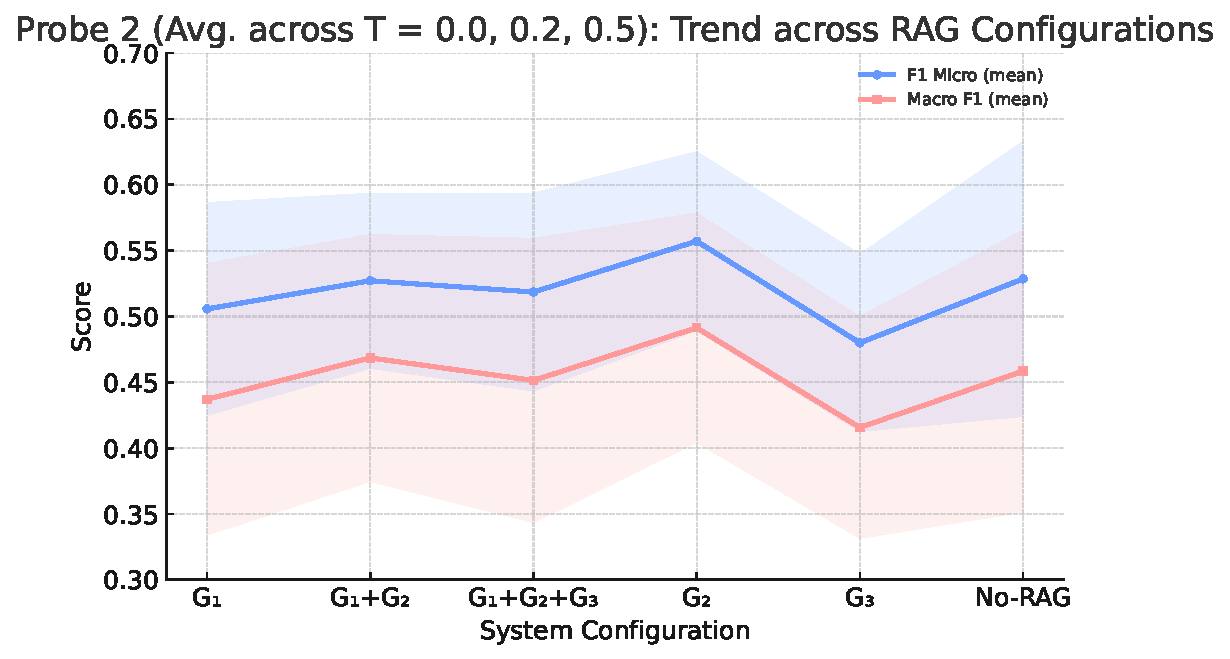
\includegraphics[width=\linewidth]{images/probe2_trend.pdf}
    \caption{Probe 2}
    \label{fig:probe2}
  \end{subfigure}
  \caption{Trends across RAG configurations for the averaged F$_1$ scores of the models in Table \ref{tab:probe1} and \ref{tab:probe2} (averaged over $T=\{0.0,0.2,0.5\}$).}
  \label{fig:probe-trends}
\end{figure*}

\subsection{Model Performance}
The models which perform well on both probes are: Anthropic Claude-3-Haiku, (which is the only non-open source model), Qwen-2.5-32B-Instruct, Llama-3.1-8B-Instruct, Llama-3.3-70B-Instruct, and GPT-OSS-20B. Llama-3.3-70B-Instruct scores the highest macro F1 on the probe 1, while Qwen-2.5-32B-Instruct has the highest macro F1 in probe 2, beating the Anthropic Claude-3-Haiku model. An observation is that these models which are particularly large in size are already trained to contain large amounts of biomedical knowledge and therefore adding external information in the shape of a domain-specific KG is likely to have very minimal value and can even cause a model to become confused and confused by irrelevant or contradictory information, shown by the dip in the results, in Table \ref{tab:probe1} and \ref{tab:probe2}. From the results, we see that normal RAG might lure in erroneous or conflicting facts, which is likely the reason why $\mathbb{G}_1$ and $\mathbb{G}_3$ fell in performance in these models. On probe 2, the image is a bit different - RAG occasionally helps. For example, the combined graph ($\mathbb{G}_1$ + $\mathbb{G}_2$ + $\mathbb{G}_3$) slightly improves Anthropic Haiku from 0.61 to 0.63 and GPT-OSS-20B from 0.46 to 0.57, suggesting that even large models can benefit from external knowledge when tackling more complex, multi-hop reasoning tasks.

Small models benefit from $\mathbb{G}_2$. The baseline scores of mistral-7B and Mixtral-8X7B are moderate (0.69 and 0.80) in probe 1 and (0.29 and 0.39) in probe 1. The performance of both probes is significantly improved when they retrieve out of the AD-oriented KG ($\mathbb{G}_2$). On probe 1 for Mixtral-8X7B, F$_1$ is increased by 0.80 to 0.89, and probe 2 F$_1$ is also increased by 0.39 to 0.51. Mistral-7B exhibited a similar behavior, from 0.69 to 0.74 for probe 1 and 0.29 to 0.33 in probe 2. Interestingly, $\mathbb{G}_1$ + $\mathbb{G}_2$ is slightly worse than $\mathbb{G}_2$ alone, indicating that the most valuable information in these models is the AD graph instead of being part of the union with T2DM knowledge. The above improvements suggest that smaller models that possess less built-in biomedical knowledge can benefit meaningfully in terms of structured biomedical knowledge to fill in the gaps in their parameter knowledge. 

Performance in $\mathbb{G}_3$ showed a downward spike, even though there was no conclusive evidence as to why. In the models, except in Mistral and Mixtral, the $\mathbb{G}_3$ graph reduces the F$_1$. An interesting case of the Llama-3.1-8B  Instruct model shows that the combined larger graph: $\mathbb{G}_1$ + $\mathbb{G}_2$ + $\mathbb{G}_3$ dropped the performance from 0.85 to 0.65 on probe 1. 0.65 was the same value as when using $\mathbb{G}_2$ alone, and was even less (0.62) on $\mathbb{G}_1$ alone.  Probe 2 was quite similar, as we saw a drop in the combined graph of  $\mathbb{G}_1$ + $\mathbb{G}_2$ + $\mathbb{G}_3$ fom 0.50 to 0.40 macro F$_1$. We hypothesized that a larger KG may add irrelevant relations, and our findings validate this, meaning that the broader graph may mislead LLMs, exposing them to unfounded relations. 

Upon adding up the improvement over the No-RAG baseline across all the models and all the probes, one can easily see that $\mathbb{G}_2$ is positive (mean improvement +0.006 F$_1$) and $\mathbb{G}_1$, $\mathbb{G}_3$ and the combination of graphs have negative mean improvements (–0.04 to -0.01). Therefore, the graph on AD ($\mathbb{G}_2$) is the only domain-specific KG that was helpful.


\section{Discussion}
\label{sec:discussion}
It is experimentally demonstrated that the source of the retrieval and the scope of retrieval $\mathbb{G}_1$, $\mathbb{G}_2$, $\mathbb{G}_3$, and their combinations directly influence the quality of answers. Since Probe 1 is derived out of $\mathbb{G}_3$, the resulting merged KG is likely to include the accurate facts sought by a large number of questions; whereas Probe 2 is created out of $\mathbb{G}_1 \cap \mathbb{G}_2$, thus signals that are similar across the two domains of diseases have a stronger influence. In both probes, the addition of additional sources ($\mathbb{G}_1$, $\mathbb{G}_2$, $\mathbb{G}_3$) does not assure higher accuracy: the addition of breadth raises recall but may introduce many other unrelated distracting facts that reduce precision.

% Put this macro in your preamble (or just above the first table):
\newcommand{\sym}[1]{\ifmmode^{#1}\else\(^{#1}\)\fi}

% ===================== Table: Probe 1 =====================
\begin{table*}[t]
  \centering
  \small
    \caption{RAG system comparison on {Probe 1}: Macro-F1 and significance vs.\ No-RAG}
    \label{tab:rag_probe1}
    \begin{tabular}{lcccccc}
      \toprule
      \textbf{Model} & \textbf{No-RAG} & $\mathbb{G}_1$ & $\mathbb{G}_2$ & $\mathbb{G}_1$+$\mathbb{G}_2$ & $\mathbb{G}_3$ & $\mathbb{G}_1$+$\mathbb{G}_2$+$\mathbb{G}_3$ \\
      \midrule
      Llama-3.1-8B-Instruct    & 0.83 & 0.67\sym{***} & 0.65\sym{**}  & 0.62\sym{***} & 0.66\sym{***} & 0.65 \\
      Mistral-7B-Instruct-v0.3 & 0.69 & 0.70           & 0.74          & 0.70           & 0.73           & 0.71 \\
      Mixtral-8$\times$7B-v0.1 & 0.80 & 0.84           & 0.89\sym{**}  & 0.80           & 0.84           & 0.87\sym{*} \\
      Qwen-2.5-32B-Instruct    & 0.91 & 0.84\sym{*}    & 0.88          & 0.89           & 0.87\sym{*}    & 0.88 \\
      GPT-OSS-20B              & 0.91 & 0.87           & 0.82\sym{*}   & 0.86\sym{*}    & 0.85\sym{*}    & 0.82 \\
      Anthropic Claude-3-Haiku & 0.91 & 0.84           & 0.93          & 0.93           & 0.90           & 0.93 \\
      Llama-3.3-70B-Instruct   & 0.96 & 0.71\sym{***}  & 0.90\sym{**}  & 0.91\sym{*}    & 0.92\sym{*}    & 0.92\sym{**} \\
      \bottomrule
    \end{tabular}

      \footnotesize
      Notes: Stars denote Welch two-sample $t$-test vs.\ No-RAG using the three replicates per condition:
      \;$\sym{*}\,p{<}.05$, \;$\sym{**}\,p{<}.01$, \;$\sym{***}\,p{<}.001$.

\end{table*}


\begin{table*}[t]
  \centering
  \small
    \caption{RAG system comparison on {Probe 2}: Macro-F1  and significance vs.\ No-RAG}
    \label{tab:rag_probe2}
    \begin{tabular}{lcccccc}
      \toprule
      \textbf{Model} & \textbf{No-RAG} & $\mathbb{G}_1$ & $\mathbb{G}_2$ & $\mathbb{G}_1$+$\mathbb{G}_2$ & $\mathbb{G}_3$ & $\mathbb{G}_1$+$\mathbb{G}_2$+$\mathbb{G}_3$     \\
      \midrule
      Llama-3.1-8B-Instruct    & 0.50 & 0.41\sym{*}  & 0.45         & 0.42\sym{*}    & 0.40\sym{*}  & 0.37\sym{**} \\
      Mistral-7B-Instruct-v0.3 & 0.29 & 0.23\sym{*}  & 0.33         & 0.29           & 0.24\sym{*}  & 0.25 \\
      Mixtral-8$\times$7B-v0.1 & 0.39 & 0.42         & 0.51\sym{*}  & 0.54\sym{*}    & 0.43         & 0.50\sym{*} \\
      Qwen-2.5-32B-Instruct    & 0.60 & 0.54\sym{**} & 0.61         & 0.55\sym{*}    & 0.48\sym{**} & 0.52\sym{**} \\
      GPT-OSS-Bb              & 0.39 & 0.45         & 0.48\sym{*}  & 0.46           & 0.41         & 0.46 \\
      Anthropic Claude-3-Haiku & 0.55 & 0.50\sym{*}  & 0.54         & 0.55           & 0.47\sym{**} & 0.57\sym{*} \\
      Llama-3.3-70B-Instruct   & 0.49 & 0.51         & 0.52         & 0.47           & 0.48         & 0.49 \\
      \bottomrule
    \end{tabular}
      \footnotesize
     
     Notes: Stars denote Welch two-sample $t$-test vs.\ No-RAG using the three replicates per condition:
      \;$\sym{*}\,p{<}.05$, \;$\sym{**}\,p{<}.01$, \;$\sym{***}\,p{<}.001$.
\end{table*}


\subsection{Significance}
We provide statistical significance of each condition (three independent runs each model-probe-system) (paired with paired two-sample $t$-tests against No-RAG): $^{*}\!p<0.05$, $^{**}\!p<0.01$, $^{***}\!p<0.001$. Table \ref{tab:rag_probe1} and \ref{tab:rag_probe2} only indicate differences that are of significance at these values; non-stars would not be statistically different to the baseline at $\alpha{=}0.05$.

\subsection{How RAG scope interacts with each probe}

\paragraph{Probe 1}
This probe was constructed out of direct existing knowledge, and systems that used $\mathbb{G}_3$ directly, accessed a single graph that happened to answer all Probe 1 facts; however, these did not help these systems, but rather introduced extraneous context, which caused failure:
\begin{itemize}
  \item Large generalist models (Llama-3.3-70B). Adding additional, tangential evidence, on the basis of $\mathbb{G}_1$ only, generated a huge, significant decline ($^{***}$), smaller, but significant, declines in the case of $\mathbb{G}_2$, $\mathbb{G}_3$, and $\mathbb{G}_1$+$\mathbb{G}_2$ ($^{*}$–$^{**}$). The model already captures a lot of knowledge that is required to respond to health-based questions.
  \item Mid-sized mixture models (Mixtral-8$\times$7B). $\mathbb{G}_2$ yields a \emph{significant} gain ($^{**}$) and $\mathbb{G}_1$+$\mathbb{G}_2$+$\mathbb{G}_3$ a smaller gain ($^{*}$), suggesting that well-scoped AD evidence helps when merged facts are relevant but not memorized.
  \item Smaller instruction models (Llama-3.1-8B). Against all KG-RAG settings, the performance is significantly low. One-sample t-test incorrect on Probe 1 ($^{*}$–$^{***}$): Sensitive to distractors in the case of retrieval of multiple semantically related facts.
  \item Other models. Mistral-7B shows no reliable change on Probe 1 (mostly unstarred), while Qwen-2.5-32B shows small but significant drops for $\mathbb{G}_1$ and $\mathbb{G}_3$ ($^{*}$).
\end{itemize}

\textbf{Why this pattern?}
Probe 1 questions reflect the merged space in existing literature, (AD\,+\,T2DM) i.e. different from just naively joining $\mathbb{G}_1$ and  $\mathbb{G}_2$. When retrieval comes from a narrower domain ($\mathbb{G}_1$ or $\mathbb{G}_2$) or an over-broad union ($\mathbb{G}_1$+$\mathbb{G}_2$+$\mathbb{G}_3$) the context either {misses} key merged relations or {dilutes} them with near-miss facts (e.g., disease-specific mechanisms that are irrelevant to the asked relation). High level models, with their substantial common-sense and medical knowledge inherent in them, can be readily diverted by near-misses. On the contrary, mid-sized models take advantage of focused AD signal ($\mathbb{G}_2$) when it coincides with merged facts of a probe.

\paragraph{Probe 2 (formulated on $\mathbb{G}_1\cap \mathbb{G}_2$).}
In this case, consistent evidence between the two diseases will be of greatest importance:
\begin{itemize}
  \item Mixtral-8$\times$7B. All of $\mathbb{G}_2$, $\mathbb{G}_1$+$\mathbb{G}_2$, $\mathbb{G}_1$+$\mathbb{G}_2$+$\mathbb{G}_3$ are improving significantly ($^{*}$), a fact that implies that AD-centric cues and their combination with T2DM are quite consistent with the intersection facts.
  \item Qwen-2.5-32B. The several settings of RAG ($\mathbb{G}_1$, $\mathbb{G}_1$+$\mathbb{G}_2$, $\mathbb{G}_3$, $\mathbb{G}_1$+$\mathbb{G}_2$+$\mathbb{G}_3$) result in important drops ($^{*}$–$^{**}$) and $\mathbb{G}_2$ is not statistically different to baseline. This indicates accuracy rather than breadth: AD-specific retrieval is less risky than the domain mixture of this probe.
  \item Mistral-7B. $\mathbb{G}_1$ and $\mathbb{G}_3$ indicate minor yet significant declines ($^{*}$); other settings are not significant.
  \item Llama-3.1-8B. The vast majority of KG-RAG environments impair performance ($^{*}$–$^{**}$), which once more indicates susceptibility to distractors in smaller models.
  \item GPT-OSS-20B \& Claude-Haiku. Mixed outcomes: some modest gains (e.g., Haiku with $\mathbb{G}_1$+$\mathbb{G}_2$+$\mathbb{G}_3$, $^{*}$) and several significant drops where the added context conflicts with the intersection signal.
  \item Llama-3.3-70B. None of the significant differences is observed- in keeping with a strong prior which is neither aided nor injured by the retrieved snippets.
\end{itemize}

\subsection{Explaining the patterns of stars}
We want to consider if the RAG is useful or harmful. There are three typical processes that we see:
\begin{enumerate}
  \item  Models are more potential to assist in the event that the construction space of the probe equals the retrieval space (Probe 1 with $\mathbb{G}_3$, Probe 2 with $\mathbb{G}_2$ or $\mathbb{G}_1$+$\mathbb{G}_2$). False positive (e.g. Probe 2 and $\mathbb{G}_3$) enhances contradictions and off-target cues and produces $^{*}$/$^{**}$ drops.
  \item  The recall is augmented by unions of ($\mathbb{G}_1$+$\mathbb{G}_2$), $\mathbb{G}_1$+$\mathbb{G}_2$)+$\mathbb{G}_3$) but it bring heterogeneous evidence to it. Otherwise, the models will overfittingly adapt to spurious but fluent responses, and will produce large drops even with truthful facts.
  \item Larger models tolerate imperfect retrieval better, (as we see in Table \ref{tab:rag_probe1} and \ref{tab:rag_probe2} where we have often unstarred or mixed effects. However, these models are also susceptible to {highly plausible} distractors; smaller models rely more heavily on retrieved text and thus amplify retrieval noise, leading to frequent $^{*}$–$^{***}$ drops.
\end{enumerate}

\subsection{Temperature effects}
System-to-system changes in temperature (0, 0.2, 0.5) had little influence on the conclusions of the RAG type: most in-system patterns were statistically insignificant, and significant ones were small compato system differences. In practice, these probes are mainly tuned by RAG choice; temperature tuning must always come second after a well-scoped graph is chosen and a strong retriever is selected.

\subsection{Frontier LLMs and Non-expert Baseline}
\label{subsec:frontier_llm_baseline}

We also posed both probes to two general-purpose LLMs and a non-expert human being. 

\begin{table}[t]
  \centering
  \scriptsize
    \caption{Gemini, ChatGPT, and non-expert human performance on Probe~1  and Probe~2.}
    \label{tab:frontier_llm_human}
    \begin{tabular}{lcc}
      \toprule
      \textbf{Agent} & \textbf{Probe 1 (100)} & \textbf{Probe 2 (110)} \\
      \midrule
      Gemini 2.5 Pro & 99/100 (99\%) & 69/110 (62.7\%) \\
      ChatGPT 5 Thinking & 98/100 (98\%) & 77/110 (70.0\%) \\
      Naive Human (no medical knowledge) & 38/100 (38\%) & 30/110 (27.3\%) \\
      \bottomrule
    \end{tabular}
\end{table}

Table~\ref{tab:frontier_llm_human} contrasts the accuracy of Gemini, ChatGPT, and a non-expert human across Probe~1 and Probe~2. Both frontier models achieve near-ceiling performance on Probe~1 (99\% and 98\%, respectively), revealing that the initial probe tasks are largely saturated. In contrast, Probe~2 introduces greater conceptual and retrieval difficulty, producing a notable accuracy decline—Gemini drops by 36.3\% points, while ChatGPT falls by 28\%. The naive human baseline shows only a modest relative decline, but its overall accuracy remains far below that of the models. The naive human baseline is a test for random guessing, as the people who took the test did not have prior knowledge of the field and were encouraged to guess randomly.

When compared with the open-weight counterparts in Tables~\ref{tab:probe1} and~\ref{tab:probe2}, the frontier models display markedly higher stability and consistency. Anthropic Claude-3-Haiku, the strongest among the smaller systems, achieved accuracies around 96\% on Probe 1 but fell to roughly 61\% on Probe 2, a pattern mirrored by all the other models. This shows that Probe~2 acts as a discriminative benchmark, separating models with generalizable reasoning (ChatGPT and Claude-tier systems) from those whose performance is more retrieval-anchored or domain-fragile.

ChatGPT’s smaller degradation indicates stronger robustness to task complexity and class imbalance, aligning with its narrower gap between Micro and Macro F$_1$ in Probe~2. Gemini’s sharper fall suggests sensitivity to rare or ambiguous cases, reinforcing that Probe~2 better exposes differential reasoning depth rather than surface-level recall. Overall, frontier LLMs far exceed human baselines, yet their relative separation on Probe~2 highlights the probe’s discriminative power for evaluating balanced generalization.

\subsection{Error Analysis}
We covered the following errors shown in Table \ref{tab:error-breakdown}: (1) {Directionality flips} (picked $B\!\to\!A$ instead of $A\!\to\!B$), (2) {Two-hop chain order errors} (mis-ordered $A\!\to\!B\!\to\!C$ pairs), (3) {Negation/exception misreads} (e.g., ``\emph{is not associated}'' / ``\emph{pick the exception}''), 
(4) {Immediate vs.\ downstream cause} (selected a true but non-proximal effect),
(5) {Undefined token guesswork} (e.g., ambiguous labels like ``FX protein'') and
(6) {Overweighting canonical AD triad} (A$\beta$/tau/neuroinflammation selected when vascular/metabolic was targeted)

\begin{table}[t]
\scriptsize
\centering
\caption{Miss classification on Probe~2 (33 total errors).}
\label{tab:error-breakdown}
\begin{tabular}{lrr}
\toprule
\textbf{Category} & \textbf{Count} & \textbf{Percent} \\
\midrule
Directionality flips & 9 & 27.27\% \\
Two-hop chain order & 8 & 24.24\% \\
Negation/exception & 6 & 18.18\% \\
Immediate vs.\ downstream & 5 & 15.15\% \\
Undefined token guesswork & 3 & 9.09\% \\
AD-triad overweighting & 2 & 6.06\% \\
\midrule
\textbf{Total} & \textbf{33} & \textbf{100\%} \\
\bottomrule
\end{tabular}
\end{table}

\subsection{Recommendations}
\begin{itemize}
  \item When adding several graphs, do so conditionally: by putting in a ranker that favors off-topic passages being demoted and evidence being given precedence that is found in both domains of the disease.
  \item Smaller models benefit most from clean, highly relevant passages, while larger models need less context overall but require stricter filtering to avoid distractors.
  \item Given three runs per condition, using star-coding ($^{*}$/$^{**}$/$^{***}$) is essential to avoid over-interpreting small differences in mean values that might not be statistically meaningful.
\end{itemize}

\paragraph{Threats to validity}
(1) Only three replicates per cell limit power; results marked unstarred could still harbor small effects. (2)  Factual mix reproducible by our KG construction decisions (entity normalization, relation filtering, and co-reference backbone) determines the factual mix that can be accessed, and any improvement or error in this regard directly translates into the results of QA. (3) Prompting and re-ranking were held fixed; stronger retrieval/re-ranking may change the balance between precision and recall.
